%!TEX root=../document.tex

\section{Ergebnisse}
\label{sec:Ergebnisse}



\subsection{Technologien}
\subsection{diff sync}
Diff synchronisation bietet die Möglichkeit mit nodejs mit einer Webseite die man zu einer Mobile Web app machen kann eine schnelle und einfache Möglichkeit an.

\subsubsection{couchbase}
Auch mittels couchbase ist es möglch die Daten zu syncronisieren.
Der NoSQL Server ist für die Verwaltung der Daten zuständig.Sync Gateway ist die Schnittstelle zw. Server und Client.Couchbase Lite ist die Client-Datenbank.\cite{couchbase}

Hier gibt es auch einen Vergleich zw. den couchbase und firebase.\\ \textit{https://db-engines.com/de/system/Couchbase\%3BFirebase+Realtime+Database}
\subsubsection{firebase}

Firebase ist eine vollständig verwaltete Plattform für den Aufbau von iOS-, Android- und Web-Apps, die unter anderem eine automatische Datensynchronisierung, Authentifizierungsdienste, Messaging, Dateispeicher und Analysen bietet.\



\begin{figure}[h]
	\centering
	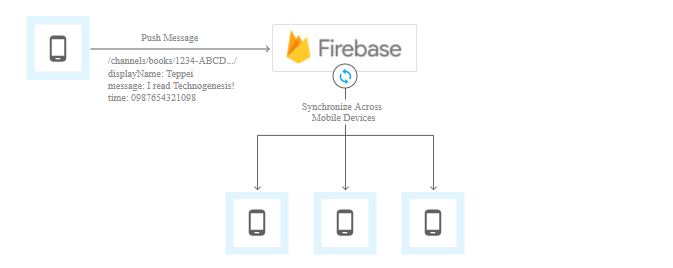
\includegraphics[width=0.7\linewidth]{images/firebase}
	\caption{firebase}
	\label{fig:firebase}
\end{figure}

Verwendet wurde das Produkt \textit{Firebase Realtime Database}. Welches die Client-Synchronisierung übernimmt.Leider bietet firebase die Replikation mit dem kostenpflichtigen Abo an.\\ Der Client sendet die Daten in der firebase Datenbank .Gespeichert wird es in einem JSON auf der Datenbank.Und Firebase synchronisiert  die Clients .


\subsection{Firebase}
Um Firebase mit Android Studio zu verbunden auf \verb|Tools -> Firebase| den Assistenten starten.
Dieser Assistent zeigt die Produkte die Firebase anbietet an.Firebase Realtime Database wurde ausgewählt, da dies die synchonistaion der Mobile abwickelt.



\begin{figure}[h]
	\begin{subfigure}[b]{0.5\textwidth}
	\centering
	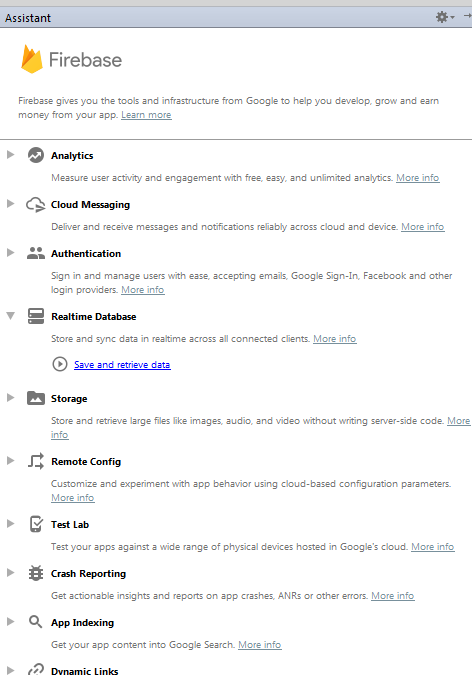
\includegraphics[width=0.7\linewidth]{images/assistent}
	\caption{firebase-assistent}
	\label{fig:assistent}
\end{subfigure}%
\begin{subfigure}[b]{0.5\textwidth}
		\centering
	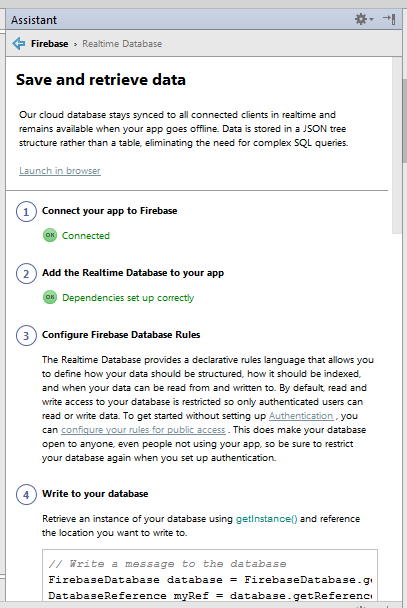
\includegraphics[width=0.7\linewidth]{images/connectedfirbase}
	\caption{firebase-assistent-step by step}
	\label{fig:connectedfirbase}
\end{subfigure}%
	
\end{figure}
Als erstes wird auf dem Button für das Connecten des Android Projekts mit firebase, dazu wird auf dem eingeloggten Google Account eine Datenbank mit dem Projektnamen aus Android erstellt.Danach werden die Dependencies runtergeladen und dem Android Projekt hinzugefügt.Nach der erfolgreichen Konfiguration von Firebase kann mit Hilfe des Guides Daten gelesen und geschrieben werden.\cite{f_readwrite}\cite{listdata}

Dabei wird eine Automatische konfigurierte Authentifizierung angeboten ,die wird ausgeschalten, da sie nicht benötigt wird.


Die Gui wurde über Drag and Drop im \textit{res/layout/activity\_main.xml} design. Eine View\_List für das Anzeigen der Elemente der Datenbank wurde gewählt und 3Buttons die ,die CRUD -Funktionalitäten darstellen.
\begin{figure}[h]
	\centering
	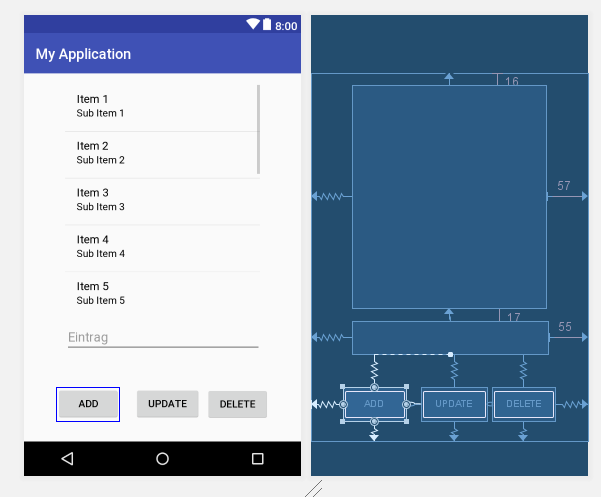
\includegraphics[width=0.7\linewidth]{images/gui}
	\caption{User Interface}
	\label{fig:gui}
\end{figure}
Die GUI-Komponenten wurden mit der \textit{MainActivity} Klasse initialisiert. Ein Array namens \textit{adapter} für die Speicherung der Elemente und Anzeige auf der View\_List wurde erstellt.Ein Listener wurde für das Selektieren von Elementen gesetzt.

\begin{lstlisting}[style=Java,caption={Gui, Adapter-Array für die Anzeige der Elemnete, Listener für die Selektion}]

	button_add = (Button) findViewById(R.id.add);
	button_update = (Button) findViewById(R.id.update);
	button_delete = (Button) findViewById(R.id.delete);
	eintrag = (EditText) findViewById(R.id.editText2);
	view = (ListView) findViewById(R.id.listview);
	
	adapter = new ArrayAdapter<String>(this,
	android.R.layout.simple_list_item_single_choice,
	listItems);
	view.setAdapter(adapter);
	view.setChoiceMode(ListView.CHOICE_MODE_SINGLE);
	
	view.setOnItemClickListener(
	new AdapterView.OnItemClickListener() {
	public void onItemClick(AdapterView<?> parent, View view, int position, long id) {
	selectedPosition = position;
	itemSelected = true;
	button_delete.setEnabled(true);
	}
	});
\end{lstlisting}

\subsection{CRUD-Funktionalitäten}
\subsubsection{Realtime Database}
\begin{lstlisting}[style=Java ,caption={datenbank Instanz und Referenz}]
FirebaseDatabase database = FirebaseDatabase.getInstance();
DatabaseReference myRef=database.getReference("list");
\end{lstlisting}


Auf den 3 Button wie vorhin erwaehnt sind die CRUD-Funktionalitaeten anwendbar.
\begin{lstlisting}[style=Java,caption={Button Listener fuer den Add_Button}]

myRef.addChildEventListener(childListener);

button_add.setOnClickListener(new View.OnClickListener() {
@Override
public void onClick(View v) {
String key = myRef.push().getKey(); //jeses Element bekommt ein unique key zugewiesen
String text = eintrag.getText().toString();

myRef.child(key).child("description").setValue(text);//wert aus Edittext wird ausgelesen und in die datenbak eingefuegt
adapter.notifyDataSetChanged();
Toast.makeText(MainActivity.this, "Inserting Data", Toast.LENGTH_SHORT).show();

}
});

\end{lstlisting}


Der add\_Button mit dem \textit{onClickListener} wird hier veranschaulicht .Es ändert sich nicht viel zu den anderen Button-Funktionalitäten.
\begin{lstlisting}[style=Java,caption={childeventListener für das einfuegen in das Adapter-array für die Anzeige}]
ChildEventListener childListener = new ChildEventListener() {
	@Override
	public void onChildAdded(DataSnapshot dataSnapshot, String s) {
		String d = dataSnapshot.child("description").getValue().toString();
		//aus der Datenbak wird das in den String geschpeichert und dem apdapter-array hinzugefuegt
		adapter.add(d);
		Toast.makeText(MainActivity.this, "list", Toast.LENGTH_SHORT).show();
		listKeys.add(dataSnapshot.getKey());
	}
\end{lstlisting}
Die dazu gehörige \textit{ChildEventListener} wird hier veranschaulicht.


\subsubsection{Offine-Verfügbarkeit}
Die Persistence wird eingeschaltet und auf die Referenz das Synchronisieren ebenfalls eingeschalten.\cite{offline}
\begin{lstlisting}[style=Java,caption={Offine-Verfügbarkeit}]
FirebaseDatabase.getInstance().setPersistenceEnabled(true);
myRef = database.getReference("list");
myRef.keepSynced(true);
\end{lstlisting}
Derzeit ist es möglich das zu testen.Leider erkennt die Applikation nach ca. 2min das sie wieder online ist. Daher könnte man dies noch verbessern.
\begin{figure}
	\centering
	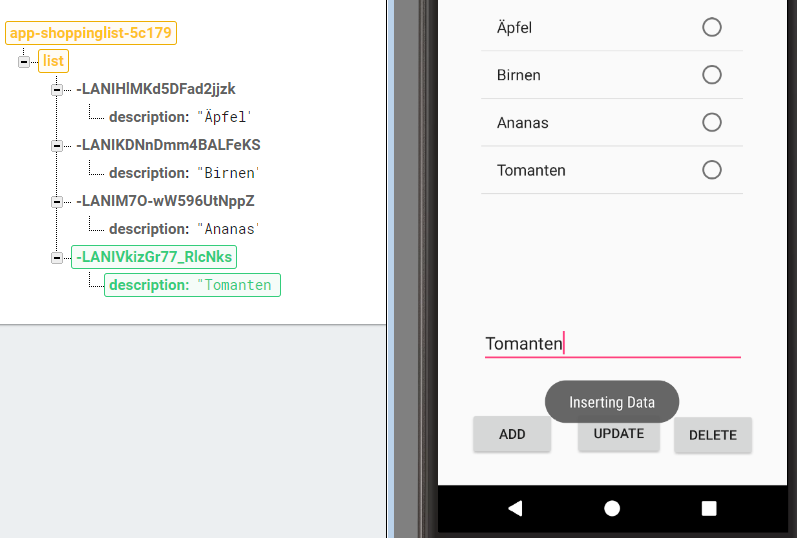
\includegraphics[width=0.7\linewidth]{images/livedemo}
	\caption{fire-Datenbank und Android-App}
	\label{fig:livedemo}
\end{figure}

Hier kann man die firebase-Datenbank sehen und die App. Die grüne Farbe ist laut legende neu Hinzugefügt.Es werden Tomanten eingefügt.Auf der App sieht man das es gerade eingefügt wird.(inserting Data).